\chapter{Inleiding}
De hedendaagse meest gebruikte database management systemen (DBMS's) zijn de relationele DBMS's of NoSQL systemen \cite{dbengine-ranking}. 

Het RDBM is er gekomen onder invloed van het artikel van E. Codd over het relationele model in 1969 \cite{codd1970relational}. Het sleutelconcept van het relationele model is dat de data georganiseerd is in relaties (tabellen) die gekoppeld zijn door middel van keys (constraints), hierbij wordt zoveel mogelijk redundante data vermeden. 
Voorbeelden van populaire relationele DBMS's (RDBMS's) zijn Oracle, MySQL en PostgreSQL. 

De NoSQL databases zijn een nieuwe generatie van systemen, de NoSQL beweging is gestart in 2000 en staat voor '\textit{Not only SQL}'. Deze systemen zijn er gekomen als reactie op het relationele model en willen meer flexibele database, lagere complexiteit, hogere doorvoer van data, horizontale schaalbaarheid en het draaien op commodity hardware.  Verschillende voorbeelden van NoSQL systemen zijn Google BigTable, Amazon Dynamo, HBase, MongoDB, ... \cite{Strauch.NoSQL} 

In de volgende sectie zullen beide systemen in meer detail aanbod komen, waarna de huidige staat voor het objectief vergelijken van de systemen aanbod. Tenslotte zal de onderzoeksvraag voor de thesis geformuleerd worden. 

\section{Relationele en NoSQL DBMS's} 
Op dit moment zijn de meest gebruikte DBMS's de relationele en NoSQL systemen, maar wat dit net inhoudt en wat de verschillen tussen beiden zijn, zal in deze sectie in meer detail aanbod komen. 

\subsection{Relationele database}
Een RDBMS is een DBMS gebaseerd op relationele model voor het structuren van de database.

Het relationele model is gebaseerd op de theoretische wiskundige principes van set-theorie en eerste-orde predicaten logica. Het model organiseert de data in tabellen en relaties tussen de tabellen. De tabel heeft kolommen die verschillende velden voorstellen en elke rij een collectie van gerelateerde datawaardes is. De relaties tussen de verschillende tabellen toont mogelijke connecties. Een belangrijke eigenschap is dat de tabellen en relaties genormaliseerd worden, hiermee wordt redundante informatie verwijderd. Dit zorgt voor een hogere data integriteit en een vermindering in data anomalieën die kunnen optreden bij een update.\cite{Elmasri:2010:FDS:1855347} \\
De normalisatie kan geïllustreerd worden met het korte voorbeeld in figuur \ref{fig:Relationeel-Model-Normalisatie}: de professor voor een vak zal bij elke student hetzelfde zijn, het veranderen van een professor voor een vak zou in het eerste geval een update van alle ingeschreven studenten inhouden, in het tweede geval is dit maar de aanpassing van een enkel record, hetzelfde geldt voor de student. \\
Interactie met de RDBMS gebeurt op basis van SQL (Structured Query Language), een taal gebaseerd op de relationele logica geeft uitgebreide query mogelijkheden aan de gebruiker van de software.   
\begin{figure}[ht!]
\centering
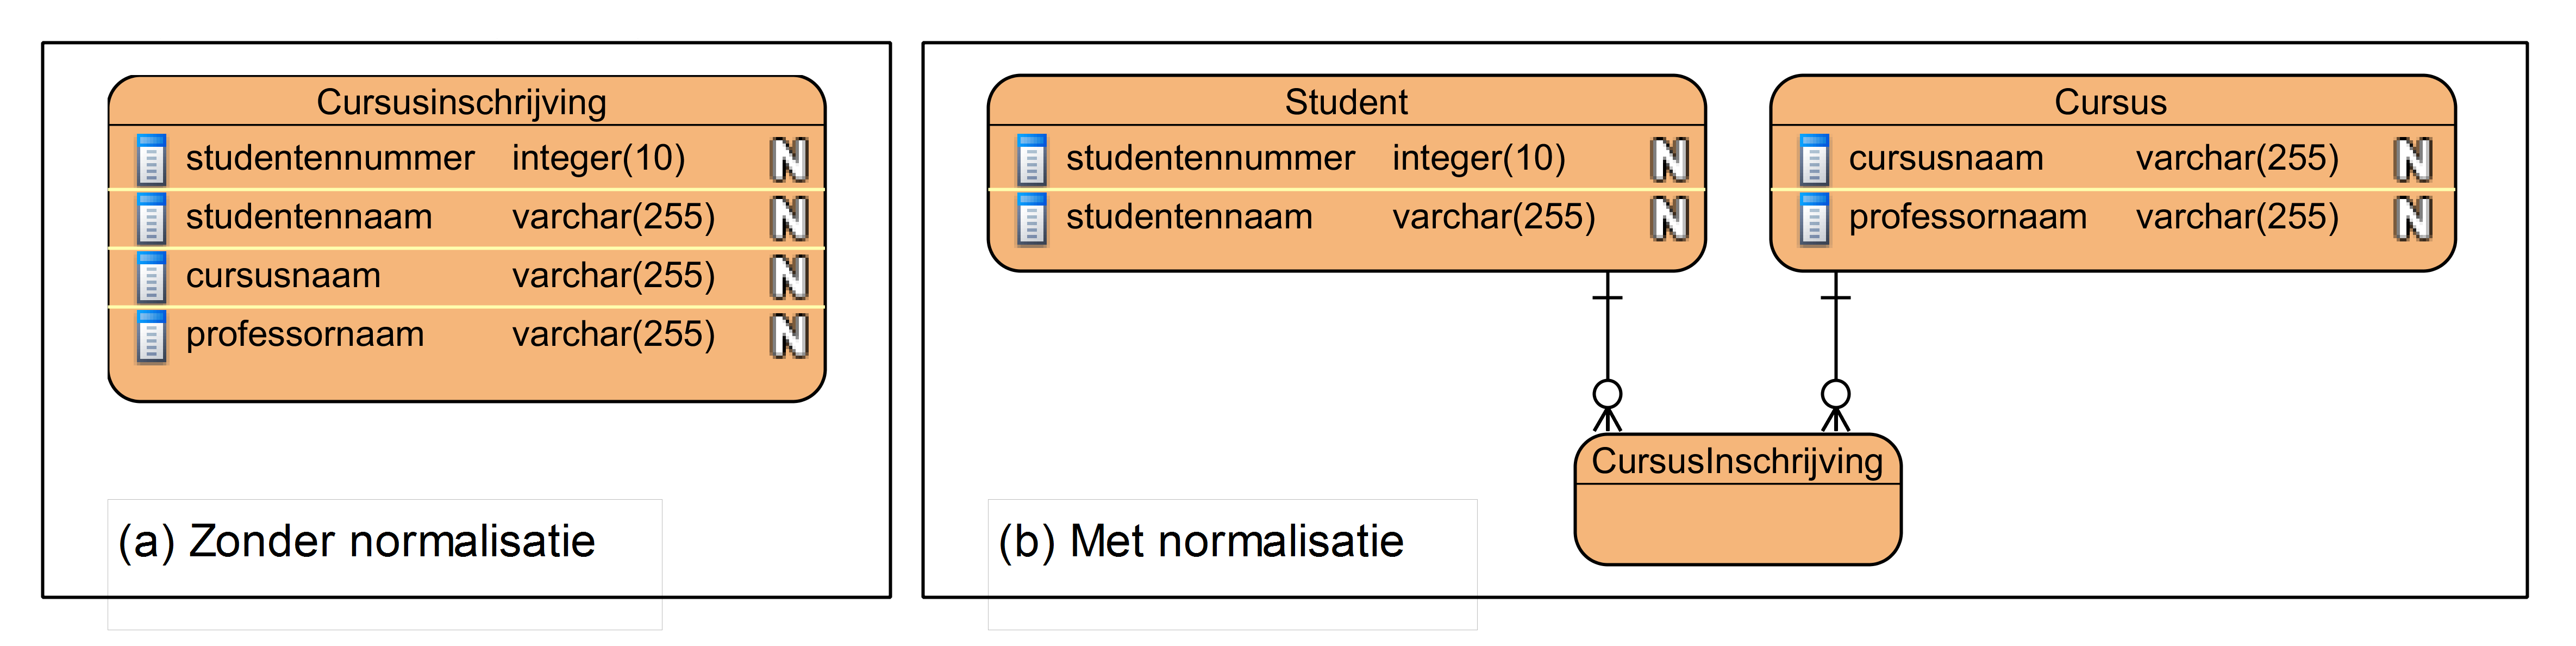
\includegraphics[width=\linewidth]{img/Relationeel-Model-Normalisatie.png}
\caption[Relationeel datamodel (a) zonder en (b) met normalisatie]{Relationeel datamodel (a) zonder en (b) met normalisatie}
\label{fig:Relationeel-Model-Normalisatie}
\end{figure}

Een belangrijk concept in een relationele database is ACID, welk tussen verschillende transacties wordt gegarandeerd:

\paragraph{Atomair (\underline{A}tomicity)} Een database transactie moet oftewel volledig uitgevoerd worden oftewel heeft geen enkele bewerking plaatsgevonden. 

\paragraph{Consistent (\underline{C}onsistency)} Een transactie behoudt de consistentie als de volledige uitvoering van de transactie de database van één consistente staat naar een andere brengt. Een consistente staat is een staat die ervoor zorgt dat waardes van een instantie consistent zijn met de andere waarden in dezelfde staat. Een voorbeeld is het overschrijven van \euro{50} van persoon A naar B, op het einde moet de totale som nog steeds gelijk zijn, A \euro{50} minder en B \euro{50} meer. Een inconsistente staat zou zijn dat enkel A \euro{50} minder heeft maar B nog steeds evenveel. 

\paragraph{Geïsoleerd (\underline{I}solation)} Een transactie moet uitgevoerd worden alsof ze geïsoleerd is van andere transacties, die eventueel gelijktijdig uitgevoerd worden. 

\paragraph{Duurzaam (\underline{D}urability)} Een voltooide transactie kan later niet ongedaan gemaakt worden.

Deze verschillende concepten bieden de gebruiker van het RDBMS garanties die de programmeur van de database kan gebruiken voor zijn systeem. Daartegen over staat wel dat dit de complexiteit van de RDBMS groeit, ook indien dit voor bepaalde toepassingen misschien niet nodig is.

\subsection{NoSQL database}\label{sec:eventualconsistency}
NoSQL DBMS zijn ontstaan als reactie op de 'one size fits all'-gedachte die RDBMS's volgen. Dit is ook zichtbaar in de NoSQL systemen, ze bestaan in verschillende variëteiten, elk met hun eigen eigenschappen en toepassingsgebied. Toch is er een rode draad te vinden tussen de verschillende systemen vergeleken met RDBMS: 
\begin{itemize}
	\item \textbf{Lagere complexiteit}: NoSQL systemen bieden minder opties en features aan dan de RDBMS omdat bepaalde applicaties enkelen nu eenmaal niet nodig hebben. Bijvoorbeeld in een sociale netwerk moet een post niet onmiddellijk beschikbaar zijn voor al de vrienden van een persoon, maar dit mag even duren.
	\item \textbf{Hogere doorvoer}: Talrijke NoSQL systemen bieden een hogere doorvoer van data aan, meestal gecombineerd met een lagere complexiteit. 
	\item \textbf{Horizontale schaalbaarheid en werkend op commodity hardware}: Waar grote RDBMS's draaien op dure high-end systemen, was het bedoeling van NoSQL databases om te werken met eenvoudige machines (commodity hardware). \\
	Horizontale schaalbaarheid staat voor het toevoegen extra machines aan een systeem voor extra resources, in tegenstelling tot verticale schaalbaarheid waar een krachtiger machine wordt gebruikt voor de opschaling. In horizontale opschaling wordt de opschaling gedaan door de data van een enkele database of tabel te verspreiden over verschillende machines die elk maar voor een deel van de data verantwoordelijk zijn en moeten opslaan.\\
	NoSQL systemen combineren deze twee elementen en bieden hierdoor een schaalbaar systeem aan met basis componenten.
	\item \textbf{Datamodel dichter bij objecten}: De meeste NoSQL systemen zijn zodanig ontworpen dat deze de vertaling van objecten naar opslag eenvoudiger maken t.o.v. RDBMS's. Waar dat RDBMS zijn ontworpen voor de object georiënteerde programmeertalen, werd er bij de ontwikkeling van NoSQL onmiddellijk hiermee rekening gehouden.  
\end{itemize}  \noindent
Deze verschillende argumenten leiden vervolgens tot BASE, een tegenreactie op ACID. \noindent 
\begin{itemize}
 \item Basis beschikbaarheid (\textbf{B}asically \textbf{Availability}): het DBMS probeert de data nog steeds beschikbaar te houden, zelf in het geval van één of meerdere falende instanties. 
 \item \textbf{S}oft State: De data moet op een bepaald moment niet volledig consistent zijn. 
 \item Eventuele consistentie (\textbf{E}ventual Consistency): De database zal na enige tijd in een consistente status uitkomen, het is mogelijk dat oudere data tijdelijk leesbaar is. Eventuele consistentie kan op zijn beurt opnieuw onderverdeeld worden in 4 categorieën \cite[slide 16]{lipcon2009design}:
 	\begin{itemize}
 		\item \textit{Read your own writes} consistentie: Ongeachte van de server waarop een gebruiker leest, zal hij zijn update onmiddellijk correct lezen. 
 		\item \textit{Session} consistentie: De gebruiker zal zijn updates onmiddellijk kunnen lezen binnen dezelfde sessie, een sessie is hierdoor meestal gelimiteerd tot een enkele database server. 
 		\item \textit{Casual} consistentie: Als een gebruiker versie X leest en vervolgens versie Y schrijft, zal elke gebruiker die versie Y leest ook versie X lezen.
 		\item \textit{Monotonic Read} consistentie: Dit levert monotone tijdsgaranties dat een gebruiker enkel recentere data versies in de toekomst zal lezen. 
 	\end{itemize}
\end{itemize}
Deze vereisten kunnen gekoppeld worden aan de CAP theorie van Erik Brewer\cite{Brewer:2000:TRD:343477.343502}. CAP zegt dat een gedistribueerd systeem maar twee van de 3 CAP elementen kan ondersteunen: consistentie, beschikbaarheid en partitie tolerantie. Met de laatste wordt bedoelt dat enkele instanties van het systeem falen maar er nog steeds een werkend systeem is. De definitie van consistentie is hier anders als bij ACID: bij CAP is er sprake van consistentie als het DBMS zich gedraagt alsof er maar een enkel kopie van de data is.

\subsubsection{Classificatie van NoSQL systemen}
Er zijn vele NoSQL systemen ontworpen gedurende de laatste jaren, elk met hun eigen variëteit, functionaliteit en populariteit. Er bestaan verschillende manieren om de systemen te classificeren, maar één van de meest gebruikte doet dit op basis de data modellering, een korte vergelijking op basis van deze bevindt zich in tabel \ref{table:selectie-classificatie}.  

\begin{table}[!h]
	\resizebox{\textwidth}{!} {
		\begin{tabular}{l l l l l l}
			\textbf{Soort} & \textbf{Performantie} & \textbf{Schaalbaarheid} & 			\textbf{Flexibiliteit} & \textbf{Complexiteit} & \textbf{Functionaliteit} \\ \hline
			Column & hoog & hoog & gematigd & laag & minimaal \\
			Document & hoog & variabel(hoog) & hoog & laag & variabel (laag) \\
			Graph & variabel & variabel & hoog & hoog & graph theory \\
			Key-Value & hoog & hoog & hoog & geen & variabel (geen) \\
		\end{tabular}
	}
	\caption{Classificatie en categorisatie van NoSQL DBMS's door Scofield en Popescu. \cite{categorizatie-sco10} \cite{categorizatie-pop10b} }
	\label{table:selectie-classificatie}
\end{table} 

\paragraph{Column Model}In een column-gebaseerd systeem wordt de data opgeslagen per kolom in plaats van de traditionele manier, per rij. Deze aanpak werd in eerste instantie gedaan voor analyse van business intelligentie. Het systeem is geïnspireerd door de paper van Google’s Bigtable \cite{chang2008bigtable}. \cite{Strauch.NoSQL}

\paragraph{Graph Model} In een grafen model, wordt de data voorgesteld en opslagen volgens de grafen theorie: knopen, lijnen en eigenschappen op de knopen en lijnen. \cite{bollacker2008freebase}.   

\paragraph{Document Model} Document systemen zijn volgens vele de volgende stap in key-value systemen, waar deze complexere structuren toe laten, dit door middel van meerdere key/value paren per element. \cite{Strauch.NoSQL} \\
Een document moet geen vaste structuur hebben maar elk document op zich kan verschillende velden hebben, dit kan bijvoorbeeld toegepast worden bij boeken. Waar een bepaald boek een recept is, kan een ander een deel zijn van een trilogie. Bij het eerste kan de kooktijd opgeslagen worden en bij de tweede een referentie naar de andere boeken. 

\paragraph{Key-Value Model} Key-Value systemen hebben een heel eenvoudig data model, data kan opgeslagen, opgevraagd en verwijderd worden op basis van een key. De informatie die in de database zit, is de waarde voor die key. \\
Met dit eenvoudig model en functionaliteit die weinig complexiteit introduceren, kan er gestreefd worden naar een hoge performantie, schaalbaarheid en flexibiliteit. \cite{Strauch.NoSQL}

\subsection{Bespreking van verschillende DBMS's}
Databases uit 4 categorieën komen verder aanbod, er is gekozen om de Graph NoSQL DBMS's niet te bespreken omdat deze gericht zijn op andere dataset dan de overige categorieën. 
\begin{itemize}
\item Column NoSQL DBMS's: Cassandra, HBase
\item Document NoSQL DBMS's: Apache CoucheDB, MongoDB
\item Key-Value NoSQL DBMS's: LightCloud (Tokyo), MemCache, Redis, Riak, Project Voldemort
\item Relationele DBMS's: MySQL, Pgpool-II (PostgreSQL)
\end{itemize}

Deze keuze van deze systemen is gebaseerd op de paper van Christophe Strauch \cite{Strauch.NoSQL}. Een korte bespreking van de verschillende systemen kan gevonden worden in appendix \ref{sec:BesprekingDBMS}.

Deze 10 systemen laten een variatie van verschillende opties zien, zowel in query mogelijkheden als naar een gedistribueerde configuratie waar er keuzes volgens het CAP theorema gemaakt moeten worden. 


\section{Objectieve vergelijking van de verschillende systemen volgens CAP}
De databasemanagementsystemen zijn voor meer dan 40 jaar actief. Met de opkomst van het relationele model in 1969 door E. Codd \cite{Codd:1970:RMD:362384.362685}, zijn gedurende vele jaren de relationele DMBS de leidende technologie geweest. Maar de afgelopen 10 jaar is er in het landschap veel veranderd met de opkomst van de NoSQL DBMS's die afstappen van het ACID naar BASE, meer gefocust op het werken op grote data in een gedistribueerde omgeving. 

Nu zijn er vele verschilpunten tussen verschillende systemen, dit gaat van het datamodel tot de verschillende keuzes in het CAP theorema. In dit gedeelte zal er gekeken worden welke methodes er al beschikbaar zijn voor het meten van de performantie, consistentie en beschikbaarheid en mogelijke resultaten. 

\subsection{Performantie benchmarking}
Indien men verschillende DBMS wilt vergelijken bestaan er al enkele tools en studies om de performantie te kunnen vergelijken, een blogpost van A. Popescu \cite{PopescuBenchmarkOverview} geeft een overzicht van verschillende benchmarking tools. 

Als eerste hebben vele DBMS's interne benchmarking tools, waarmee de database op verschillende configuraties kan getest en vergeleken worden. Deze resultaten zijn nuttig indien het DBMS al gekozen is en men bezig is met het aanpassen van de parameters of om te onderzoeken wat net de bottleneck is in een bepaald systeem. Een voorbeeld hiervan is mongoperf\footnote{\url{http://docs.mongodb.org/manual/reference/program/mongoperf/}} voor MongoDB. 

Andere studies focussen op het testen van verschillende systemen en daarbij kunnen verschillende doelstellingen zijn: het ontwikkelen van een breed toepasbare tool, het testen van een grote verscheidenheid van DBMS's of het testen van een specifieke categorie van systemen. Elke van deze benchmarking brengt extra kennis bij maar heeft ook zijn beperkingen. Het totaal pakket van al de testen kan een gebruiker de informatie geven om een beter gefundeerde keuze te maken. 

De eerste categorie, het \textbf{ontwikkelen van een tool} voor verschillende systemen, heeft als grote voordeel dat andere gebruikers nadien de testen opnieuw kunnen uitvoeren met de systemen in hun configuratie. Het is namelijk niet gegarandeerd dat het resultaat van een jaar geleden met de nieuwste versie nog te vergelijken is.
Het grootste nadeel is het type testen dat kan uitgevoerd worden, er is een grote variëteit aan systemen elk met hun eigen datastructuur en query mogelijkheden. De tool moet dus een gemeenschappelijke subset zoeken en enkel dit soort queries kunnen getest worden. Een voorbeeld van een dergelijke tool de opensource tool YCSB\cite{cooper2010benchmarking}. In deze tool kan elk DBMS's getest worden zolang een basisset van 5 queries kan implementeren: het invoegen, updaten, verwijderen en opvragen van een enkel record met daarnaast ook de mogelijkheid tot scan queries, met behulp van 1 query een verzameling van records tegelijk op te vragen. \\
Sommige systemen ondersteunen bepaalde queries niet onmiddellijk maar bevatten wel de functionaliteit om deze via een omweg te implementeren, bijvoorbeeld een update kan geïmplementeerd worden door het opvragen, verwijderen en vervolgen invoegen van het geüpdatete record. 

Een volgende categorie zijn de \textbf{resultaten van gerelateerde DBMS's}, in deze categorie zijn er voornamelijk resultaten te vinden van systemen met hetzelfde datamodel. Het grote voordeel hieraan is dat deze systemen in de meeste gevallen een vrij gelijkaardige set aan query mogelijkheden bevatten waardoor er meer diepgang is dan tussen meer verschillende systemen. Een voorbeeld van zulk onderzoek is gedaan door P. Pirzadeh et al\cite{pirzadeh2011performance} voor de key-value systemen, meer specifiek is er gefocust op het uitvoeren van range queries tussen Cassandra, HBase en Voldemort. Hoewel in de categorisatie van deze thesis de eerste twee onder column NoSQL vallen, zijn deze nog vrij gelijklopend. \\
In deze categorie vallen ook de resultaten die meestal getoond worden op de website van de DBMS's, een vergelijkende benchmark met andere soortgelijke systemen. Hoewel de resultaten niet altijd volledig objectief zijn, kan de gevolgde test methode wel interessant zijn. Een voorbeeld van deze studie is de Key-Value benchmarking van VoltDB\cite{huggkey} waar Cassandra en VoltDB vergeleken worden, een belangrijke kanttekening is dat de auteur zelf al aanhaalt dat de systemen vrij verschillend zijn zoals appels en appelsienen.  

Als laatste categorie, zijn er de \textbf{resultaten van verschillende DBMS's} waar zeer verscheidene systemen met elkaar getest worden. De belangrijkste voordeel is dat er resultaten zijn die verschillende soorten met elkaar vergelijken en waardoor niet alleen verschillen in het datamodel kunnen vergeleken worden in toekomstige studies maar ook performantie verschillen. Het nadeel is ook hier dat er een gemeenschappelijke subset gevonden moet worden, hierdoor kunnen bepaalde databases hun kracht net niet laten zien. Verschillende van deze onderzoeken zijn \cite{tudorica2011comparison} en \cite{rabl2012solving}. Deze laatste maakt gebruik van de YCSB tool die hierboven besproken was. 


\subsection{Consistentie testen}
Er is al relatief veel onderzoek gebeurd naar de performantie van de verschillende systemen. Maar daarnaast is er ook de consistentie eigenschappen die verschillend kunnen zijn. 

Een recent artikel \cite{golab2014eventually} (maart 2014), begint met het stellen dat er momenteel nauwelijks gekwantificeerde methodes bestaan om de eventuele consistente te meten. In hun artikel stellen zij twee mogelijke methoden voor: de actieve of passieve analyse. \\
De \textbf{actieve} analyse bestaat het wegschrijven van data in een database waarna 1 of meerdere andere gebruikers meten hoe lang het duurt vooraleer zij de nieuwe waarde lezen. 
De \textbf{passieve} analyse wordt er gekeken hoe de gebruiker handelt met het systeem en hoe de data updates zich gedragen. Leest deze altijd de laatste waarde (=strikte consistentie)? Is het mogelijk dat een nieuwe waarde al wordt gelezen voor de schrijfactie voltooid is? \\
Beide systemen hebben hun eigenschappen, de actieve analyse kan gezien worden als een systeem georiënteerde analyse, test hoe lang het duurt voor de data beschikbaar is over de verschillende systemen en heeft als uitkomst hoe DBMS's zich verschillend gedragen ten opzichte van elkaar of in verschillende netwerk- en hardwareomgevingen. 
Bij de passieve analyse is georiënteerd naar de gebruiker toe, hoe moet deze zijn toepassingen aanpassen, wat zijn specifieke eigenschappen van het systeem? 

Voor beide analyse methodes is er al onderzoek gebeurd, maar het meeste is gebeurd naar de actieve analyse. Onder andere Duitse onderzoekers hebben op het Amazon S3 platform getest hoe lang het duurt vooraleer data geschreven in MiniStorage, een database systeem, beschikbaar is voor alle gebruikers. \cite{bermbach2011eventual}. \\
Daarnaast zijn er ook 2 interessante resultaten gevonden: allereerst heeft het Amazon S3 systeem geen monotone lees consistentie, daarnaast bleek het inconsistentie interval voor een bepaald record periodiek verloop te hebben dat niet door de onderzoekers verklaard konden worden. 

De YCSB software van hierboven is door onderzoekers in de VS uitgebreid naar YCSB++\cite{patil2011ycsb++} waardoor deze meer ondersteuning heeft om het meten van systeembelasting maar ook voor de consistentie eigenschappen. Hoewel enkele van de systemen die zij testen in principe strikt consistent zijn zoals HBase, worden deze eventueel consistent door het gebruiken van buffers bij de gebruiker. Vervolgens testen zij hoe lang het duurt voor de data ook gelezen kan worden. Een probleem met deze methode is dat deze vertraging sterk afhankelijk is van het aantal acties van de schrijvende gebruiker: indien er meer geschreven wordt, zal de buffer sneller verzonden worden naar de server en dus sneller beschikbaar zijn voor andere gebruikers. \\
Hoewel zij stellen dat er ook testen zijn gedaan naar eventuele consistentie voor Cassandra en MongoDB, zijn de resultaten niet beschikbaar in het artikel of op de website. 

Andere onderzoeker\cite{wada2011data} hebben passieve analyse uitgevoerd en gekeken hoe lang het duurt vooraleer databases in de cloud infrastructuur consistente data hebben, met een focus op Amazon SimpleDB. Er zijn testen uitgevoerd hoe lang het duurt vooraleer de meest recente data gelezen zal worden door een gebruiker. 

Bij Netflix heeft men aan passieve analyse gedaan op hun Cassandra systeem \cite{kalantzisnetflix} waar zij in hun testen geen consistentie problemen vonden naar de gebruiker toe. Er is geen vermelding hoeveel vertraging er zit tussen beide transacties. Volgens hun gaat het meer om de perceptie dat data verkeerd kan gelezen worden en de angst van het middle management. 

\subsection{Beschikbaarheidstesten}
Een derde verschilpunt is hoe de systemen omgaan met het falen van een enkele server en dit onder verschillende opties: Het is mogelijk dat deze tijdelijk uitgeschakeld wordt wegens onderhoud, het kan om een onverwachte crash van het DBMS's gaan of zelfs een hele server, tenslotte kunnen er ook nog netwerkproblemen optreden waardaar deze (tijdelijk) niet beschikbaar is. 

Nu hoe gaan deze systemen om het falen en terug online brengen van de systemen: zijn er geen acties mogelijk op de server, worden de connecties tijdelijk verbroken, is er een verhoogde of verlaagde vertraging op de transacties? En detecteert het systeem automatisch wanneer de oorspronkelijke server terug online komt of moet gemeld worden om de server terug te gebruiken? In een NoSQL DBMS waar gewerkt wordt commodity hardware, zal het falen regelmatig gebeuren en verschillende systemen reageren anders op deze acties. 

Voor informatie over hoe de verschillende systemen reageren, is het momenteel uitzoeken op de website van de software verdeler en zelf uittesten van het gedrag. Naar mijn onderzoek, bestaat er nog geen vergelijkende studie tussen de verschillende systemen. 

\section{Conclusie}
Er bestaan verschillende soorten DBMS's met verschillende mogelijkheden categorisatie. Uit de literatuur studie blijkt dat er een gebrek aan gekwantificeerd methodes is om de systemen te testen naar consistentie en beschikbaarheid. 

Het doel van deze thesis is om een methode te beschrijven die beide elementen kan testen en te implementeren. Het sofware pakket dat de testen uitvoert, zal openbaar gemaakt worden zodat anderen de resultaten kunnen vergelijken en uitvoeren op hun eigen systemen. 

Tenslotte zullen deze testen uitgevoerd worden op verschillende DBMS's om bewijs aan te leveren dat de methode werkt en al eerste initiële conclusies te kunnen trekken, die later verder kunnen ontwikkeld worden. 